% Per-shot EEG during naturalistic film: a four-perspective developmental review
% Trends in Cognitive Sciences (Cell Press) Forum Review submission
% Generated from the Markdown manuscript by manuscript:manuscript-formatting (pandoc + post-processing).

\documentclass[preprint,12pt]{elsarticle}

\usepackage[utf8]{inputenc}
\usepackage{lmodern}
\usepackage[T1]{fontenc}
\usepackage{graphicx}
\usepackage{xcolor}
\usepackage{tcolorbox}
\tcbuselibrary{breakable}
\usepackage{hyperref}
\hypersetup{colorlinks=true,linkcolor=black,urlcolor=blue,citecolor=blue}
\usepackage{natbib}
\bibliographystyle{elsarticle-num}

\title{Per-shot EEG during naturalistic film: a four-perspective developmental review}

\author[1]{Seyed Yahya Shirazi\corref{cor1}}
\ead{shirazi@ieee.org}
\cortext[cor1]{Corresponding author}

\affiliation[1]{organization={Open Science Collective},country={USA}}

\begin{document}

\begin{frontmatter}

\begin{highlights}
  \item Naturalistic EEG has shifted from whole-clip ISC to shot-locked spectral metrics
  \item Psychophysics, action, language, emotion diverge on per-shot EEG predictions
  \item Language-model regressors cannot transfer to silent character animation
  \item Per-shot EEG ERSP in children viewing animation has no published precedent
  \item HBN-EEG Release 3 sits at this empty intersection and can test the predictions
\end{highlights}

\begin{abstract}
Naturalistic-stimulus neuroscience has moved from whole-clip inter-subject correlation (ISC) to event-locked methods that interrogate individual shots. Most empirical evidence is adult functional magnetic resonance imaging (fMRI), adult intracranial electroencephalography (iEEG), or adult scalp electroencephalography (EEG) ISC. Per-shot event-related spectral perturbation (ERSP) in a developmental cohort viewing silent character animation has no published precedent. We review the corpus that constrains this design space and argue that psychophysics, action, language, and emotion make divergent, partly-falsifiable predictions about the 0 to 500 ms post-shot-onset window. The Healthy Brain Network EEG Release 3 cohort viewing \textit{The Present} (Pixar 2014) sits at this empty intersection, although the local 100 Hz cohort caps beta-band and gamma-band claims pending a 500 Hz validation.
\end{abstract}

\end{frontmatter}

\section{Introduction: the per-shot turn}

Naturalistic-stimulus neuroscience moved from controlled gratings to feature films in two waves. The first wave was functional. Hasson and colleagues showed that voxel-level cortical activity synchronises across viewers of the same audiovisual movie in up to 45 percent of cortex during free functional magnetic resonance imaging (fMRI) viewing \cite{Hasson2004IntersubjectSO}. The second wave was electrophysiological. Correlated-component analysis on scalp electroencephalography (EEG) demonstrated that engagement, attention, memory, and audience preference all scale with the reliability of stimulus-locked variance \cite{dmochowski2012correlated,Ki2016AttentionSM,Cohen2016MemorableAN,Dmochowski2014AudiencePA,Madsen2022CognitivePO}. A third wave is now emerging that interrogates individual events within the continuous stream. Nentwich and colleagues recorded 6328 contacts in 23 patients across 43.6 minutes of film clips, regressed responses against optical-flow magnitude, saccade onsets, and film-cut onsets simultaneously, and found whole-brain shot-cut transients with semantic novelty modulation \cite{Nentwich2023SemanticNM}. The hippocampus distinguishes within-event camera cuts from across-event narrative boundaries \cite{Ben-Yakov2018TheHF}, and event-segmentation theory frames boundaries as moments of high prediction error with hierarchical timescales mapped from sensory cortex to default-mode regions \cite{zacks2007event,speer2007narrative,baldassano2017event}.

A separate developmental tradition has used Pixar shorts in fMRI to map theory of mind (ToM) and pain networks in children as young as three \cite{Richardson2018DevelopmentOT} and silent abstract animation to improve magnetic resonance imaging (MRI) compliance and reveal reliable network-level activity \cite{Vanderwal2015InscapesAM}. Cross-sectional EEG inter-subject correlation (ISC) across ages 6 to 44 is the closest electrophysiological developmental anchor; ISC is highest in children and declines into adulthood \cite{Petroni2018TheVO}. None of these traditions has reported per-shot event-related spectral perturbation (ERSP) at the 0 to 500 ms post-onset window in a child cohort viewing animation.

This review argues that four research perspectives, psychophysics, action, language, and emotion, make divergent and partly-falsifiable predictions about this empty cell. The methods footprint is small: partial out log luminance ratio (LLR), accept independent component analysis-only artifact rejection because the Healthy Brain Network EEG (HBN-EEG) Release 3 cohort has no synchronous eye tracker, and pre-register a topographic-and-band rejection region before opening the data. Sections 2 to 6 develop the four perspectives in order. Section 7 synthesises them into a pre-registerable rejection region. Box 1 anchors the argument to the HBN-EEG Release 3 cohort viewing \textit{The Present} (Pixar 2014).

\section{The four-perspective scaffold}

The four-perspective scaffold is structural rather than decorative. Each perspective makes a different \textit{kind} of prediction. Psychophysics names a regressor of no interest that must be partialled before any social claim can be defended; the regressor is LLR, with motion energy as a named follow-up. Action names a band-and-topography prediction: mu-band event-related desynchronisation (ERD) over central rolandic cortex, inherited from adult mirror-system work \cite{hari1998action,pineda2005mu} but never tested in animated agents. Language names a method that structurally cannot transfer (language-model surprisal aligned to spoken transcripts) plus a positive sub-thread of silent-narrative findings that does transfer (Castelli's Heider-Simmel triangle paradigm \cite{castelli2000heider}, Vanderwal's Inscapes \cite{Vanderwal2015InscapesAM}, Naci's Hitchcock excerpt \cite{Naci2014ACN}, Lankinen's silent-visual MEG ISC \cite{Lankinen2014IntersubjectCO}). Emotion names two predictions at incompatible latencies: early occipital alpha desynchronisation and later frontal-asymmetric alpha. The four perspectives form a hierarchy of prior-evidence depth that the data can rerank.

Two themes anchor the analytic backbone independent of perspective. Theme 1, inter-subject correlation as a reliability metric, originated in fMRI \cite{Hasson2004IntersubjectSO} and migrated to scalp EEG \cite{dmochowski2012correlated}, MEG \cite{Lankinen2014IntersubjectCO}, peripheral physiology \cite{Madsen2022CognitivePO}, and audience prediction \cite{Dmochowski2014AudiencePA}. Theme 2, event segmentation, anchors in event-segmentation theory and hidden-Markov-model event-state recovery \cite{zacks2007event,baldassano2017event,speer2007narrative,Ben-Yakov2018TheHF}. The four perspectives then sit in specific corners of the theme space. Psychophysics owns Themes 4 (low-level feature regressors) \cite{Adelson1985SpatiotemporalEM,Carandini2011NormalizationAA,Nishimoto2011ReconstructingVE}, 5 (time-resolved EEG and MEG), and 11 (free-viewing EEG with eye coregistration). Action owns Themes 6 (mu rhythm and action observation) \cite{hari1998action,pineda2005mu} and 8 (social cognition through biological motion), and contributes to Themes 2 and 14 (distributed multivariate signatures). Language owns Theme 9 (LMs as regressors) \cite{Goldstein2022SharedCP,Caucheteux2022BrainsAA} as a structural comparator and Theme 10 (audiovisual integration); the silent-narrative sub-thread cuts across Themes 8 and 13 (developmental neuroimaging in cinematic paradigms). Emotion owns Themes 7 (affective dynamics), 12 (pet, animal, and baby-schema affective response), and 13. Theme 15 (predictive processing) unifies across perspectives: it ties mu-band ERD to mirror-system prediction error, LM surprisal to next-word prediction, and event boundaries to prediction-error transients. Theme 3 (naturalness gradient; Figure 2) places the stimulus on a continuum from controlled gratings to live-action film, with character animation as the intermediate point that motivates the empty-cell framing.

Perspective overlap is intentional rather than residual. The four perspectives interact at the per-shot ERSP level rather than partitioning variance cleanly. Sections 3 to 6 develop them in order, naming the band-by-topography signature each makes and the falsification region attached to each (Figure 4). Section 7 closes by combining the four rejection regions into a single pre-registerable test before group analysis. Section 3 begins with psychophysics because the bottom-up floor must be cleared before any higher-order claim can be defended.

\section{Psychophysics: the bottom-up floor}

Psychophysics anchors the bottom-up floor that every per-shot analysis must clear before claiming a higher-order effect. The lineage runs from primary visual cortex receptive fields \cite{Hubel1962ReceptiveFB} and divisive normalisation \cite{Carandini2011NormalizationAA} through natural-image statistics and spatiotemporal energy \cite{Bell1997TheC,Simoncelli2001NaturalIS,Adelson1985SpatiotemporalEM} to middle-temporal motion machinery \cite{Born2005StructureAF,Bartels2008NaturalVR}. Nishimoto and colleagues reconstructed natural movies from blood-oxygen-level-dependent activity in occipitotemporal cortex using a motion-energy front end derived from Adelson and Bergen \cite{Nishimoto2011ReconstructingVE}. The reconstruction is an existence proof that an Adelson-Bergen feature bank suffices to recover the stimulus from neural activity. Clinical visual evoked potential work supports a reliable scalp signature for luminance and contrast steps with magnocellular and parvocellular pathway assignment \cite{Tobimatsu2006StudiesOH}.

The closest electrophysiological analogue to per-shot ERSP during naturalistic film is the intracranial electroencephalography (iEEG) study of Nentwich and colleagues, who showed that motion outranks luminance for occipitoparietal cortex when triple-regressed against optical-flow magnitude, saccade onsets, and film-cut onsets \cite{Nentwich2023SemanticNM}. That result establishes a quantitative ranking among low-level regressors: per-shot LLR is one of several low-level features that need accounting. EEG ISC at the whole-clip scale tracks low-level features at occipital electrodes more strongly than higher-order content \cite{dmochowski2012correlated,Madsen2022CognitivePO,Cohen2016MemorableAN}, although attention strongly modulates this baseline \cite{Ki2016AttentionSM}. An envelope-only auditory control isolating low-level acoustic structure from higher-level musical structure \cite{Kaneshiro2021InterSubjectEC} is the methodological template the LLR-as-covariate plan inherits.

A second class of bottom-up drivers operates through the eye. Free-viewing EEG depends on eye-movement coregistration to separate stimulus-onset responses from saccade-locked and fixation-related potentials [Dimigen2011CoregistrationOE; Plöchl2012CombiningEA], and regression deconvolution of overlapping events is the methodological state of the art \cite{Dimigen2021RegressionbasedAO}. Gaze coherence varies with stimulus class, highest on Hollywood trailers and lowest on natural movie clips and static images \cite{Dorr2010VariabilityOE}; a Pixar short sits between these extremes. The HBN-EEG Release 3 cohort carries no synchronous eye tracker, which means a per-shot analysis cannot deconvolve overlapping saccade-locked transients from shot-onset responses. Independent component analysis (ICA)-based artifact rejection through adaptive mixture ICA (AMICA) and IC classification (ICLabel) is the operating compromise \cite{Bell1997TheC}. The implication for per-shot ERSP is asymmetric: per-shot LLR is the minimum partialling for any social-content claim. Motion energy computed offline from the stimulus video is the named first follow-up regressor \cite{Nishimoto2011ReconstructingVE,Nentwich2023SemanticNM}. The multivariate temporal response function (mTRF) toolbox supplies the production regression framework \cite{Crosse2016TheMT}. Figure 2 places the empty cell on the naturalness gradient.

\section{Action: mu-band ERD and event segmentation}

The action perspective makes the most specific positive prediction in the 0 to 500 ms ERSP window. Hari and colleagues showed by magnetoencephalography (MEG) that primary motor cortex is activated during passive observation of hand action via 15 to 25 Hz rolandic rebound suppression that reaches 31 to 46 percent of execution-related suppression \cite{hari1998action}. Pineda framed the EEG mu rhythm (8 to 13 Hz over electrodes C3, Cz, and C4) as a non-invasive proxy for human mirror-system engagement \cite{pineda2005mu}. Mu suppression magnitude during action observation correlates with self-reported social skill across neurotypical adults \cite{oberman2007mirror}. Lesion-symptom mapping places posterior superior temporal sulcus (STS) and ventral premotor cortex as causally necessary nodes for biological-motion perception \cite{saygin2007sts,johansson1973biological}. Predictive-coding reformulations recast mirror responses as scaling with prediction error over goal and intention \cite{kilner2007predictive,rizzolatti2004mirror,iacoboni2009mirror}. The mirror-system framing has well-known critiques outside the corpus, in particular Hickok-style objections that mu suppression also reflects general attention to moving stimuli rather than a one-to-one mirror-system signature; the absence of these critiques inside the corpus tempers the weight that the action prediction can carry.

Even with that tempering, the prediction is specific. Shots dominated by character action should produce ERD in the mu band over central electrodes, with possible beta-band rebound suppression. The Heider-Simmel tradition shows that even abstract triangle animations recruit posterior STS, medial prefrontal cortex, and temporal poles when motion implies intention \cite{castelli2000heider}. The naturalness gradient places character animation between abstract Heider-Simmel and live-action \cite{hasson2010natural}. The inferential bridge from triangle-animation fMRI activation to character-animation mu-band EEG ERD is plausible and untested at scalp-EEG resolution.

The second action beat is event segmentation. Speer and colleagues found posterior cingulate, middle-temporal, and posterior STS boundary-locked transients in fMRI during narrative listening \cite{speer2007narrative}. Baldassano and colleagues recovered a hierarchy of event boundaries from Sherlock-movie fMRI using hidden Markov models, with hippocampal boundary signals predicting subsequent free recall \cite{baldassano2017event}. Lerner and colleagues mapped temporal receptive windows from sensory cortex (milliseconds) to default-mode regions (tens of seconds) \cite{lerner2011temporal}. Chen and colleagues showed event-specific patterns in the default-mode network are shared across viewers and reactivated at recall \cite{chen2017shared}. Ben-Yakov and Henson distinguished within-event camera cuts, which produce minimal hippocampal responses, from across-event narrative boundaries, which produce robust ones \cite{Ben-Yakov2018TheHF}. Magliano and Zacks supplied the behavioural foundation that viewers segment edited films along cuts independent of dialogue \cite{Magliano2011TheIO}.

A third action beat concerns single-agent versus two-agent shots. Sliwa and Freiwald documented a dedicated cortical network in macaque for processing two-agent social interaction, separable from single-agent action perception \cite{sliwa2017macaque}. This motivates excluding two-agent shots from a clean single-agent contrast, since the social-interaction network may dominate two-agent variance.

\section{Language: comparator of non-transfer plus silent-narrative sub-thread}

\subsection{5a. Language-model regressors are structurally non-transferable}

The contemporary methodological mainstream in naturalistic neuroimaging is built around transformer-based language-model (LM) regressors aligned to spoken or read transcripts. Goldstein and colleagues showed pre-onset prediction, post-onset surprise, and contextual-embedding signatures shared between word-by-word electrocorticography (ECoG) and autoregressive LMs \cite{Goldstein2022SharedCP}. Each signature depends on speech-onset alignment. Heilbron and colleagues separated lexical, syntactic, and semantic surprisal regressors during MEG audiobook listening, all derived from LMs with word-onset alignment \cite{Heilbron2020AHO}. Caucheteux and colleagues mapped transformer intermediate layers to fMRI and MEG responses to natural narrative \cite{Caucheteux2022BrainsAA} and a cortical hierarchy of prediction timescales \cite{Caucheteux2023EvidenceOA}. Antonello and colleagues documented log-linear scaling of brain prediction with LM parameter count up to 30B \cite{Antonello2023ScalingLF}. Schrimpf and colleagues showed that next-word-prediction quality drives brain score on fMRI, ECoG, and reading-time benchmarks \cite{schrimpf2021the}. Toneva and Wehbe used BERT to predict reading fMRI and MEG, with attention-head ablations linking brain prediction to natural-language processing performance \cite{toneva2019interpreting}. Huth and colleagues built the canonical voxelwise word-embedding encoding atlas tiling cortex with semantic clusters; this method requires spoken transcripts \cite{Huth2016NaturalSR}. Nelson and colleagues tracked open-node count during syntactic merge using intracranial high-gamma dynamics, explicitly reading-based \cite{Nelson2017NeurophysiologicalDO}. The N400 family bridges to picture-context paradigms at the cost of dynamic stimulus \cite{Kutas2011ThirtyYA,DeLong2005ProbabilisticWP}.

Each method depends on word-level alignment to spoken or read stimuli. \textit{The Present} is wordless. All seven Category G cards in our language ontology (and 12 cards corpus-wide) carry \texttt{transfer-to-silent: no}. A vision-side analogue, multimodal vision-language model embeddings or scene-difference deep-network features as continuous regressors, does not yet exist in the corpus for scalp-EEG ERSP. The Lipkin frontotemporal language-network atlas \cite{Lipkin2022ProbabilisticAF} is used as the negative-control region of interest in the falsification region of Section 7.

\subsection{5b. Silent-narrative neural correlates that do transfer}

Silent-narrative neural correlates do transfer to scalp-EEG ERSP analysis even when language-model regressors cannot. Castelli and colleagues showed that silent geometric-shape animations engage medial prefrontal cortex, the temporo-parietal junction, and the STS when motion implies social interaction, with no speech required \cite{castelli2000heider}; the same paradigm in autism shows reduced engagement \cite{Castelli2002AutismAS}. Vanderwal and colleagues built Inscapes, a purpose-built silent abstract animation that improves MRI compliance and produces reliable network-level activity, used by the HBN cohort itself \cite{Vanderwal2015InscapesAM}. Naci and colleagues used a Hitchcock excerpt as a covert assessment, showing that high-order cortex can be probed from a near-silent narrative \cite{Naci2014ACN}. Lankinen and colleagues report source-space MEG reliable across viewers in occipital and temporal cortex during silent-visual and audiovisual movie conditions, the closest electrophysiological analogue with a deliberate silent-visual condition \cite{Lankinen2014IntersubjectCO}. The Studyforrest infrastructure provides an audio-only foundation that has been extended to silent-cohort contrasts \cite{Hanke2014AH7}. Schroeder and colleagues described modality-general delta- and theta-band phase alignment to attended event onsets, providing the mechanistic frame for shot-onset ERSP independent of speech \cite{Schroeder2009LowfrequencyNO}. Senkowski and colleagues described transient gamma synchronisation and low-frequency phase coupling for cross-modal binding \cite{Senkowski2008CrossmodalBT}. Van Wassenhove and colleagues showed visible mouth movements speed the auditory N1 and P2 components, an effect that does not transfer because \textit{The Present} contains no dialogue \cite{Wassenhove2005VisualSS}. Buckner, Simony, Yeshurun, Mar, and Tamir developed the default-mode network (DMN) as narrative integrator, with framing context driving within-stimulus divergence \cite{Buckner2008TheBD,Simony2016DynamicRO,Yeshurun2017SameSD,Mar2011TheNB,Tamir2016ReadingFA}.

The language perspective plays two roles. The 5a sub-thread isolates the silent-stimulus design from the dominant LM-as-regressor framework. The 5b sub-thread supplies the cortical substrates that silent narrative engages: medial prefrontal cortex, the temporo-parietal junction, the STS, and the DMN. Their independent-component-cluster analogues in EEG are the search regions for the per-shot ERSP analysis. Figure 3 makes the gap structure explicit.

\section{Emotion: two predictions at different latencies}

The emotion perspective makes two predictions with different latencies and different implicated structures. The first is an early visual-cortex emotion-schema response. Kragel and colleagues built EmoNet, a deep-learning model showing that emotion schemas are encoded in early visual cortex, predicting that emotion-tuned visual representations should appear in early-latency occipital ERSP \cite{Kragel2018EmotionSA}. Saarimaki and colleagues decoded six basic emotions during emotional movie viewing using fMRI multi-voxel pattern analysis [Saarimäki2016DiscreteNS]; Cowen and Keltner extended the taxonomy to 27 distinguishable categories from short videos \cite{Cowen2017SelfreportC2}. Distributed-network meta-analysis argues for distributed signatures over strict regional localisation \cite{Lindquist2012TheBB}, with the neurologic pain signature as a methodological exemplar of multivariate signatures of affect \cite{Wager2013AnFN}. The closest EEG correlate at the 0 to 500 ms scale is early occipital alpha desynchronisation (80 to 300 ms post-shot-onset, extrapolated from static-picture latencies). Codispoti and colleagues (2023) review the EEG alpha-band literature on emotional picture perception and conclude that alpha desynchronisation is a robust correlate of attentional engagement by emotional stimuli, with parametric arousal modulation \cite{Codispoti2023AlphabandOA}. Whether this transfers to dynamic naturalistic stimuli at sub-second timescales in a child cohort is untested.

The second prediction is a longer-latency cuteness or affiliative response. Stoeckel and colleagues reported common activation across child and dog spanning emotion, reward, affiliation, visual processing, and social cognition regions in adult mothers viewing photographs of own child versus own dog \cite{Stoeckel2014PatternsOB}. Glocker and colleagues showed that baby schema parametrically modulates nucleus accumbens reward in adults \cite{Glocker2009BabySM}. Borgi and colleagues demonstrated that children aged 3 to 6 already show parametric cuteness ratings and gaze bias for human infant, puppy, and kitten faces \cite{Borgi2014BabySI}; this is the behavioural anchor that the cuteness response is established well before adolescence. The interpretation implication is that Stoeckel measures identity-level pair-bonding and Borgi measures generic baby schema. HBN viewers have no identity-level bond with an animated puppy, so the relevant inference is from generic baby schema rather than pair-bonding circuitry.

Two EEG routes connect these predictions to observables. The first is early occipital alpha-band desynchronisation (80 to 300 ms) as an arousal-modulated correlate of attentional engagement \cite{Codispoti2023AlphabandOA}. The second is later frontal alpha asymmetry (200 to 500 ms; extrapolated downward from the seconds-to-minutes Davidson tradition) as an approach-withdrawal index \cite{Davidson2000AffectiveSP,Coan2004FrontalEA}. An updated meta-analytic critique documents smaller effect sizes and substantial reliability concerns \cite{Reznik2018FrontalAA}. The corpus contains no card applying asymmetry analysis to per-event sub-second windows during a continuous naturalistic stimulus, and none in a developmental cohort viewing film. Frontal asymmetry at shot-onset latency is therefore exploratory rather than confirmatory.

The third emotion beat is social cognition. Richardson and colleagues documented theory-of-mind and pain networks present from age three and refining with age, using Pixar shorts in 122 children \cite{Richardson2018DevelopmentOT}; this is the load-bearing developmental anchor. Mar synthesised narrative comprehension as a social-cognitive activity \cite{Mar2011TheNB}; Singer and colleagues documented affective pain-region engagement during observed pain \cite{Singer2004EmpathyFP}; Zaki and Ochsner formalised the tripartite empathy model bridging experience sharing and mental-state attribution \cite{Zaki2012TheNO}. Nummenmaa and colleagues showed emotion intensity modulates ISC in midline cortex during film viewing \cite{Nummenmaa2012EmotionsPS}; Schmaelzle and Grall theorised ISC as audience captivation [Schmälzle2020TheCB]. Two predictions sit at incompatible latencies and topographies; an LLR-partialled per-shot generalised linear model (GLM) adjudicates between them.

\section{Synthesis: integration, falsifiability, and open questions}

\subsection{7.1 Integration}

The four perspectives rank by depth of prior evidence. Psychophysics has the deepest precedent and the simplest operationalisation: partial LLR, optionally motion energy, before any condition claim. Action has the deepest specific oscillatory prediction (mu-band ERD over central rolandic clusters) but no animated-agent precedent in EEG. Language is structurally non-transferable for LM regressors but supplies cortical priors for silent narrative through its 5b sub-thread (medial prefrontal cortex, the temporo-parietal junction, the STS, the default-mode network). Emotion supplies two predictions: early occipital alpha desynchronisation \cite{Codispoti2023AlphabandOA,Kragel2018EmotionSA} and later frontal-asymmetric alpha \cite{Davidson2000AffectiveSP}, with the cuteness response anchored developmentally by Borgi \cite{Borgi2014BabySI}. Distributed-multivariate-signature framing supports IC-cluster-level analyses over single-IC decoding \cite{Lindquist2012TheBB,chen2017shared}. Figure 4 displays the four predictions in tabular form.

\subsection{7.2 Anchor case}

External precedent: Petroni and colleagues recorded 64-channel EEG at 500 Hz from 114 viewers across ages 6 to 44 during passive viewing of six naturalistic videos including animated and live-action shorts \cite{Petroni2018TheVO}. They did not analyse shot-onset ERSP and did not factor stimulus-side regressors, but they demonstrated that scalp-EEG signal exists during developmental naturalistic viewing of short videos. They are the closest external existence proof that the measurement class is feasible in adjacent territory. Internal feasibility: a partly-validated developmental EEG pipeline on HBN-EEG Release 3 brings 184 subjects through Brain Imaging Data Structure (BIDS) import, 1 Hz high-pass filtering, conditional cleanline gated by Nyquist, \texttt{clean\_rawdata} channel rejection, AMICA decomposition, ICLabel classification, dipole fitting, and \texttt{std\_precomp} ERSP precomputation; the operating constraint is that the local working set is 100 Hz, with a 500 Hz validation pass on the full Amazon S3 R3 release scheduled after pipeline validation. The two anchor assertions are independent and not interchangeable.

\subsection{7.3 Falsifiability}

A topographic-and-band rejection region for the four-perspective ranking can be pre-registered before group analysis. A surviving central-rolandic mu-band cluster (electrodes C3, Cz, and C4; 8 to 13 Hz) confirms the action prediction. A surviving frontal-asymmetric alpha cluster (electrodes F3 and F4; 8 to 13 Hz) confirms the emotion prediction. A surviving cluster in left frontotemporal IC space, overlapping the Lipkin language-network atlas \cite{Lipkin2022ProbabilisticAF} used as a negative-control mask, falsifies the four-perspective ranking by relocating the surviving signal into a perspective the thesis says should not transfer. A null result on the LLR-partialled GLM at a pre-registered cluster-level alpha (p < 0.05 corrected by mass-univariate cluster-based permutation, with the mTRF toolbox precedent \cite{Crosse2016TheMT}) also falsifies the four-perspective ranking, by localising per-shot ERSP variance entirely to bottom-up features in this cohort. Pinning the rejection region before data analysis is the publication discipline that constrains analyst degrees of freedom.

\subsection{7.4 Open questions and limitations}

Narrative position is a within-stimulus confound. Boy-only and puppy-only shots in \textit{The Present} differ on three-act position: boy-only clusters in the early-act setup, puppy-only in the late-act resolution. Any boy-vs-puppy ERSP difference may therefore be confounded with prediction-error or arousal trajectories. The response is to add shot-index-in-narrative as a continuous covariate in the group GLM and to fit a within-act stratified analysis as a named follow-up \cite{Magliano2011TheIO,baldassano2017event,chen2017shared}. Beyond narrative position, several gaps in the corpus limit what this review can claim. The Hickok-style mu-system critique is not represented in our cards, which weakens the action prediction. Klin and colleagues showed that toddlers with autism orient to audiovisual contingency rather than upright biological motion \cite{klin2009biological} and that adolescents with autism fixate eyes 50 percent as often during emotionally evocative viewing \cite{klin2002visual}; the HBN cohort includes a substantial autism-spectrum subsample, so autism status is a candidate moderator, but stratified analyses (autism-spectrum, attention, social skill) are exploratory follow-ups rather than primary tests. The emotion literature is predominantly adult; the three pet-evoked affective cards are fMRI or behavioural, not EEG. Frontal asymmetry at sub-second timescales is unprecedented and reliability-limited. The single-stimulus design forbids generalisation beyond \textit{The Present}. The 100 Hz local working set caps beta-band and gamma-band claims until the 500 Hz validation pass. The Outstanding Questions Box collects the forward-looking adjudication targets.

\begin{tcolorbox}[colback=yellow!5!white,colframe=black!50,title=Box 1: HBN-EEG Release 3 as the anchor cohort,breakable]
The Healthy Brain Network EEG (HBN-EEG) Release 3 cohort recruits 5- to 21-year-old participants in a developmental research setting and records 128-channel HydroCel Geodesic Sensor Net during passive viewing of the 3.5-minute Pixar short \textit{The Present} (2014). The local working set used in our pipeline development is 184 subjects at 100 Hz Biosignal Data Format (BDF), a Nyquist-aware downsample of the original 500 Hz. The 56 stimulus-side shots carry per-shot @@PH1@@\_temp@@, @@PH1@@\_temp@@, @@PH1@@\_temp@@, @@PH1@@\_temp@@, and @@PH1@@\_temp@@ annotations. After invalidating 3 high-drift rows (@@PH1@@\_temp@@), 49 rows are trusted, yielding 20 boy-only and 15 puppy-only shots for the mutually exclusive single-agent contrast. The pipeline runs BIDS import, 1 Hz high-pass filter, conditional cleanline (gated by Nyquist), @@PH1@@\_temp@@ channel rejection, AMICA, ICLabel (brain threshold 0.69), dipfit5, and @@PH1@@\_temp@@ ERSP. The anchor case rests on Petroni and colleagues 2018 \cite{Petroni2018TheVO} as the external precedent and this partly-validated pipeline as the internal feasibility proof.
\end{tcolorbox}

\begin{tcolorbox}[colback=blue!5!white,colframe=blue!40,title=Trends Box: recent developments enabling the per-shot framing,breakable]
Recent advances make the per-shot framing newly tractable.

\begin{itemize}
  \item \textbf{Whole-brain shot-cut response in adult intracranial EEG.} Nentwich and colleagues 2023 recorded 6328 contacts in 23 patients across 43.6 minutes of film clips and regressed responses against optical-flow magnitude, saccade onsets, and film-cut onsets simultaneously, finding whole-brain saccade- and cut-locked responses with motion concentrated in occipitoparietal cortex \cite{Nentwich2023SemanticNM}.
  \item \textbf{Hidden Markov model recovery of event states from fMRI.} Baldassano and colleagues 2017 recovered a hierarchy of event boundaries from Sherlock-movie fMRI, with hippocampal boundary signals predicting subsequent free recall \cite{baldassano2017event}.
  \item \textbf{Cross-sectional developmental EEG-ISC.} Petroni and colleagues 2018 reported whole-clip EEG-ISC reliability across ages 6 to 44 during passive viewing of six naturalistic videos, peaking in childhood \cite{Petroni2018TheVO}.
  \item \textbf{Silent abstract animation for MRI compliance.} Vanderwal and colleagues 2015 built Inscapes, used by HBN itself, with reliable network-level activity \cite{Vanderwal2015InscapesAM}.
  \item \textbf{Multi-level cinematic-feature regression.} Kauttonen and colleagues 2015 regressed multi-level cinematic features against fMRI ISC, supplying a methodological template for shot-level feature annotation \cite{Kauttonen2015OptimizingMF}.
  \item \textbf{Open developmental EEG releases.} HBN-EEG and Studyforrest \cite{Hanke2014AH7} make large-N developmental datasets available for naturalistic-stimulus analysis at unprecedented scale.
\end{itemize}
\end{tcolorbox}

\begin{tcolorbox}[colback=green!5!white,colframe=green!40!black,title=Outstanding Questions,breakable]
\begin{enumerate}
  \item Does per-shot EEG spectral perturbation in a developmental cohort viewing silent animation survive partialling for log luminance ratio and motion energy at the 0 to 500 ms window?
  \item Is mu-band ERD over central rolandic clusters elicited by animated-character action observation, as it is by hand-action observation in adults?
  \item Does cuteness-driven affective response in children produce a sub-second EEG signature distinguishable from generic arousal in the alpha band, and is the signature compatible with frontal asymmetry at sub-second timescales given the meta-analytic reliability concerns?
  \item Can a topographic-and-band rejection region for the four-perspective ranking be pre-registered before group analysis, and is the central-rolandic-versus-frontal-asymmetric-versus-language-network discrimination operationalisable from EEG IC clusters?
  \item Can a multimodal vision-language embedding regressor substitute for language-model surprisal on silent stimuli?
  \item Does within-stimulus narrative position (three-act trajectory) explain condition-level effects that survive low-level partialling in single-stimulus designs?
  \item What is the residual saccade-locked variance contamination in shot-onset EEG ERSP without a synchronous eye tracker, and at what cohort size does ICA-only artifact rejection become sufficient?
\end{enumerate}
\end{tcolorbox}

\section*{Glossary}
\begin{description}
  \item[\textbf{Event-related spectral perturbation (ERSP)..}] A time-frequency representation of the change in spectral power (and optionally inter-trial phase coherence) at each frequency and latency relative to an event, computed by averaging single-trial power spectrograms after subtracting a baseline window.
  \item[\textbf{Inter-subject correlation (ISC)..}] The Pearson correlation between time courses of different participants viewing the same stimulus, computed voxel-wise (fMRI) or component-wise (EEG and MEG); a stimulus-locked reliability metric.
  \item[\textbf{Log luminance ratio (LLR)..}] The base-10 logarithm of the ratio of mean luminance in the first post-shot frame to the mean luminance in the last pre-shot frame; a per-shot stimulus-side regressor of the visual transient at shot onset.
  \item[\textbf{Adaptive mixture independent component analysis (AMICA)..}] A multi-model extension of ICA that estimates a mixture of ICA decompositions, used in EEGLAB-style pipelines for artifact-resistant source separation.
  \item[\textbf{IC classification (ICLabel)..}] An automated classifier that labels independent components as brain, muscle, eye, heart, line noise, channel noise, or other.
  \item[\textbf{Mu rhythm..}] An 8 to 13 Hz oscillation over central rolandic electrodes (C3, Cz, C4) that desynchronises during motor execution and during observation of others' actions.
  \item[\textbf{Event-related desynchronisation (ERD)..}] A decrease in spectral power in a specific frequency band time-locked to an event, interpreted as cortical activation in the band's reference resting state.
  \item[\textbf{Frontal alpha asymmetry..}] The difference between right and left frontal alpha-band (8 to 13 Hz) power, traditionally framed as an approach-withdrawal index; recent meta-analyses report smaller effects and reliability concerns.
  \item[\textbf{Default-mode network (DMN)..}] A set of cortical regions including medial prefrontal cortex, posterior cingulate cortex, and lateral parietal cortex that show coordinated activity during internally directed cognition, narrative comprehension, and rest.
  \item[\textbf{Theory of mind (ToM)..}] The cognitive capacity to attribute mental states (beliefs, desires, intentions) to self and others.
  \item[\textbf{Temporal response function (TRF)..}] A linear filter that maps a continuous stimulus feature to a continuous neural response, fit via regularised regression.
  \item[\textbf{Baby schema..}] A set of infantile physical features (large head, large eyes, round cheeks) that elicit attentional, affective, and caregiving responses.
  \item[\textbf{Naturalistic stimulus..}] A continuous, ecologically valid stimulus (typically a film, audiobook, or video game) presented without trial-by-trial structuring. Naturalness is a continuum from controlled gratings to live-action film, with character animation and abstract Heider-Simmel triangles as intermediate points (Figure 2).
  \item[\textbf{Event segmentation..}] The cognitive process of parsing continuous experience into discrete events at moments of high prediction error, organised hierarchically.
  \item[\textbf{Temporal receptive window..}] The span of preceding time over which a brain region integrates information; ranges from milliseconds in primary sensory cortex to tens of seconds in default-mode regions.
\end{description}

\clearpage
\section*{Figures}

\begin{figure}[h!]
  \centering
  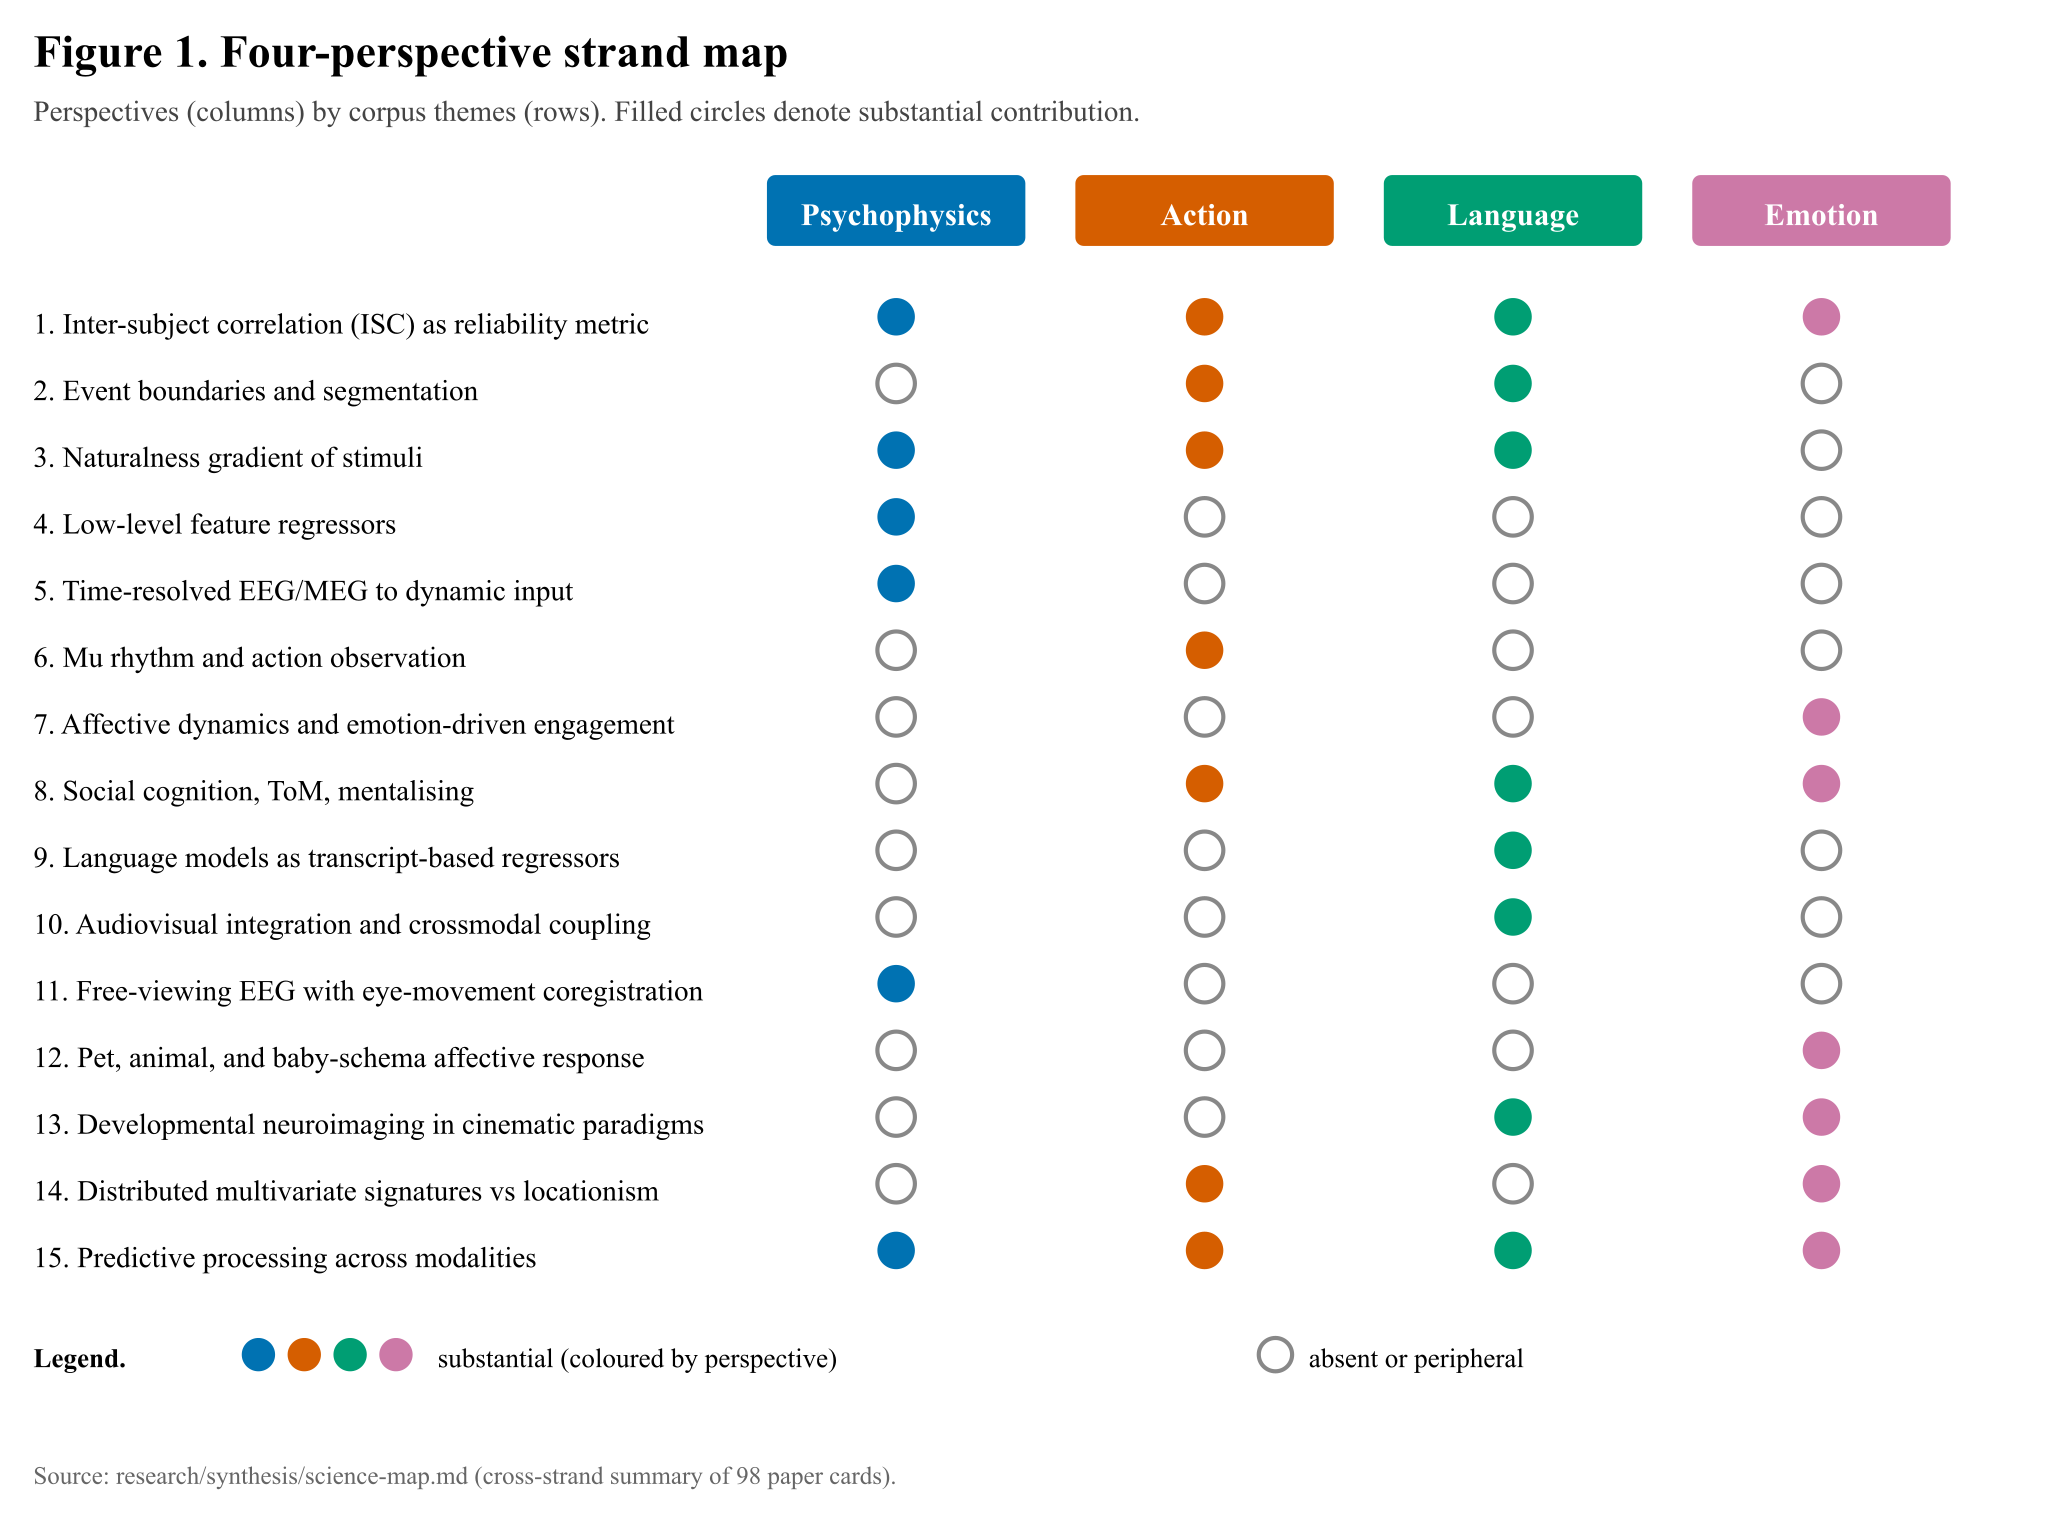
\includegraphics[width=\textwidth]{figures/fig1.png}
  \caption{\textbf{Four-perspective strand map.} Four research perspectives (psychophysics, action, language, emotion) mapped against 15 corpus themes. Filled coloured circles indicate substantial contribution from the perspective to the theme; outlined circles indicate absence or peripheral relevance. The four columns are colour-coded by perspective and the legend doubles as a colour key. Theme overlap is intentional: the perspectives interact at the per-shot ERSP level rather than partitioning variance cleanly.}
  \label{fig:strand-map}
\end{figure}

\begin{figure}[h!]
  \centering
  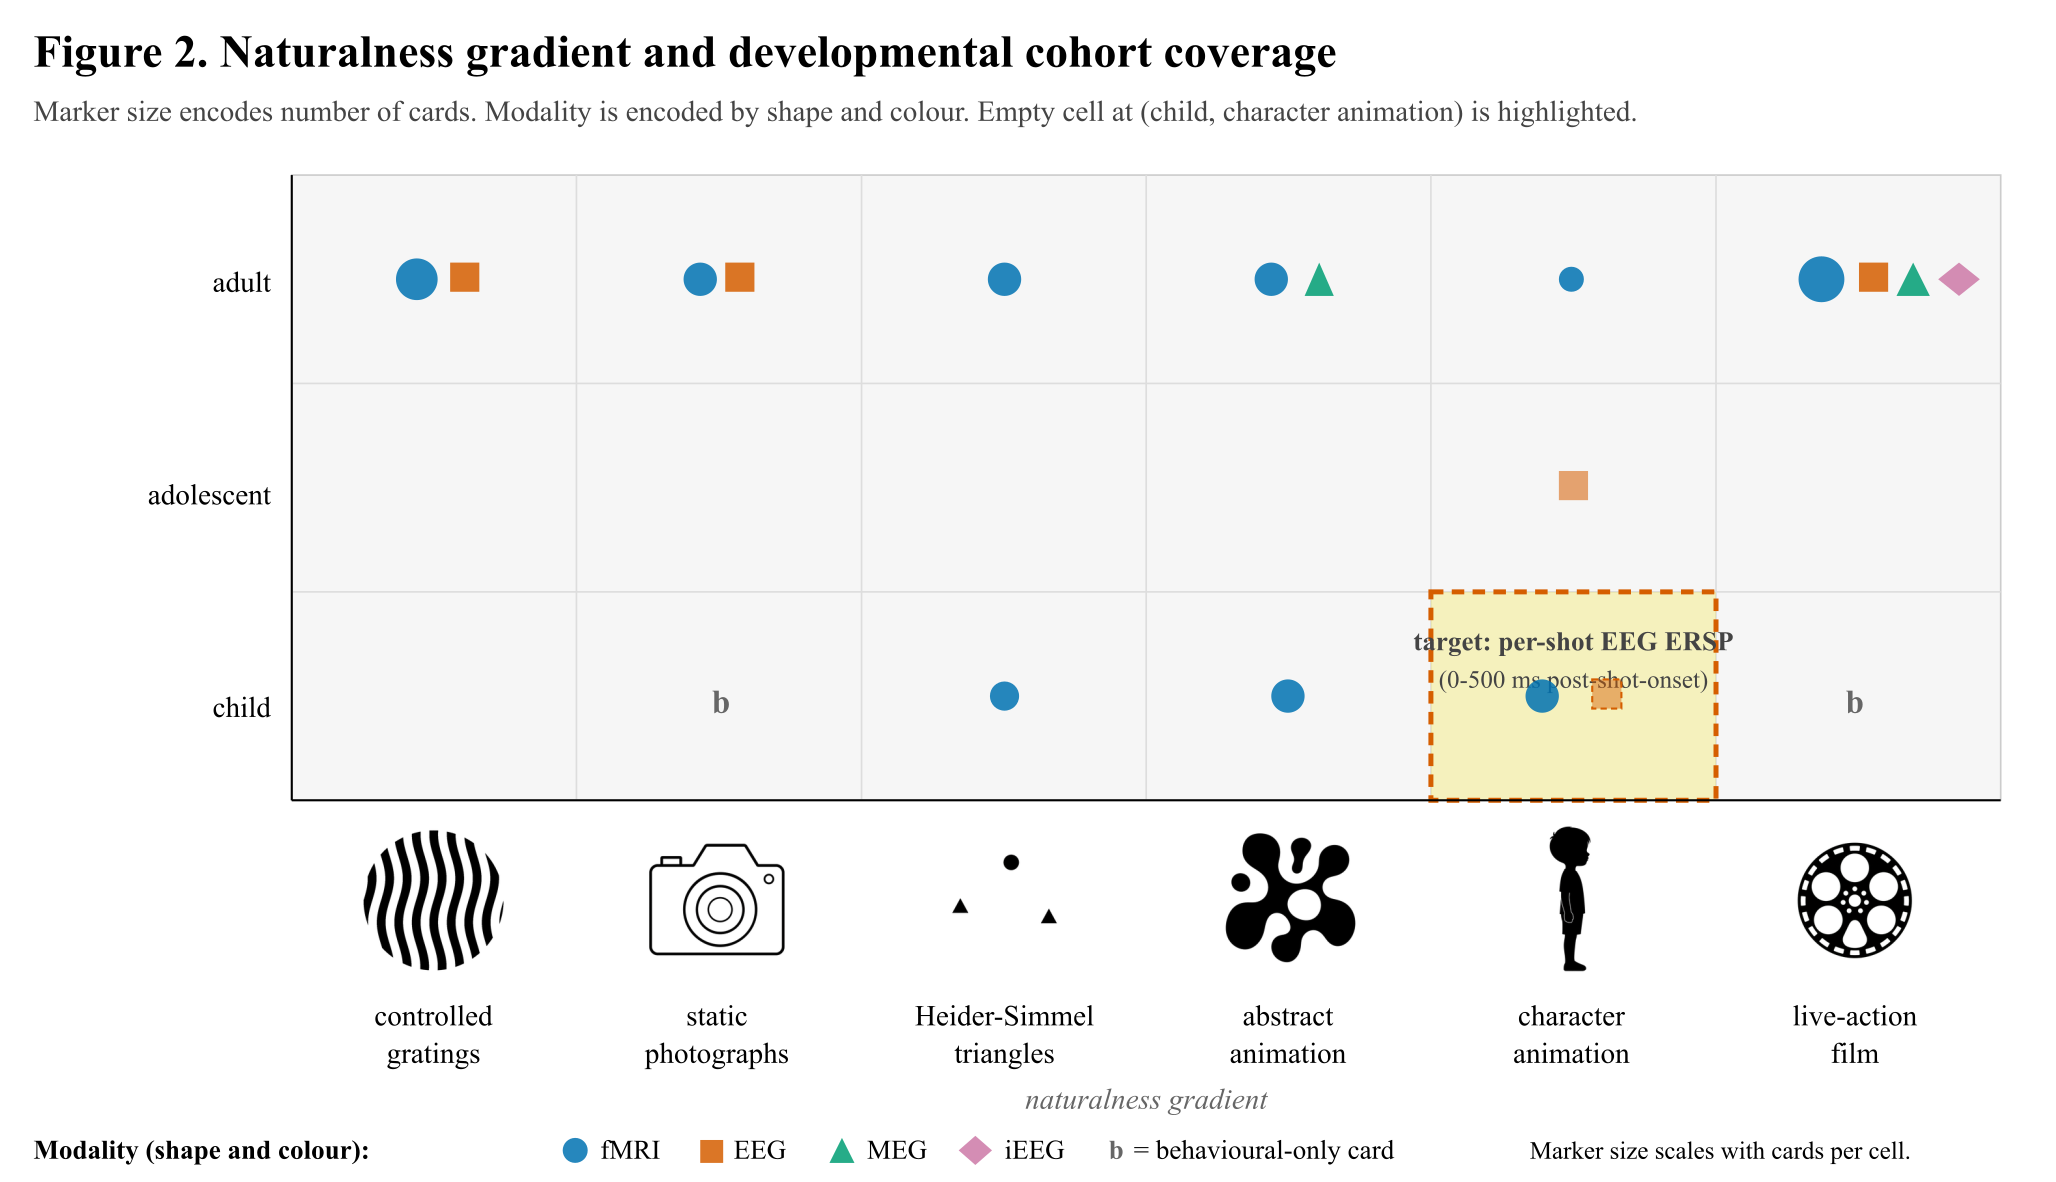
\includegraphics[width=\textwidth]{figures/fig2.png}
  \caption{\textbf{Naturalness gradient and developmental cohort coverage.} Stimulus naturalness on the x-axis (controlled gratings, static photographs, Heider-Simmel triangles, abstract animation, character animation, live-action film) versus participant cohort on the y-axis (adult, adolescent, child). Markers are sized by number of corpus cards and shaped and coloured by modality (fMRI as circle, EEG as square, MEG as triangle, intracranial EEG as diamond; behavioural-only entries as the letter b). The dashed yellow rectangle at (child, character animation) marks the target cell for per-shot EEG ERSP at the 0 to 500 ms window: existing coverage is whole-clip ISC, not per-shot ERSP.}
  \label{fig:naturalness}
\end{figure}

\begin{figure}[h!]
  \centering
  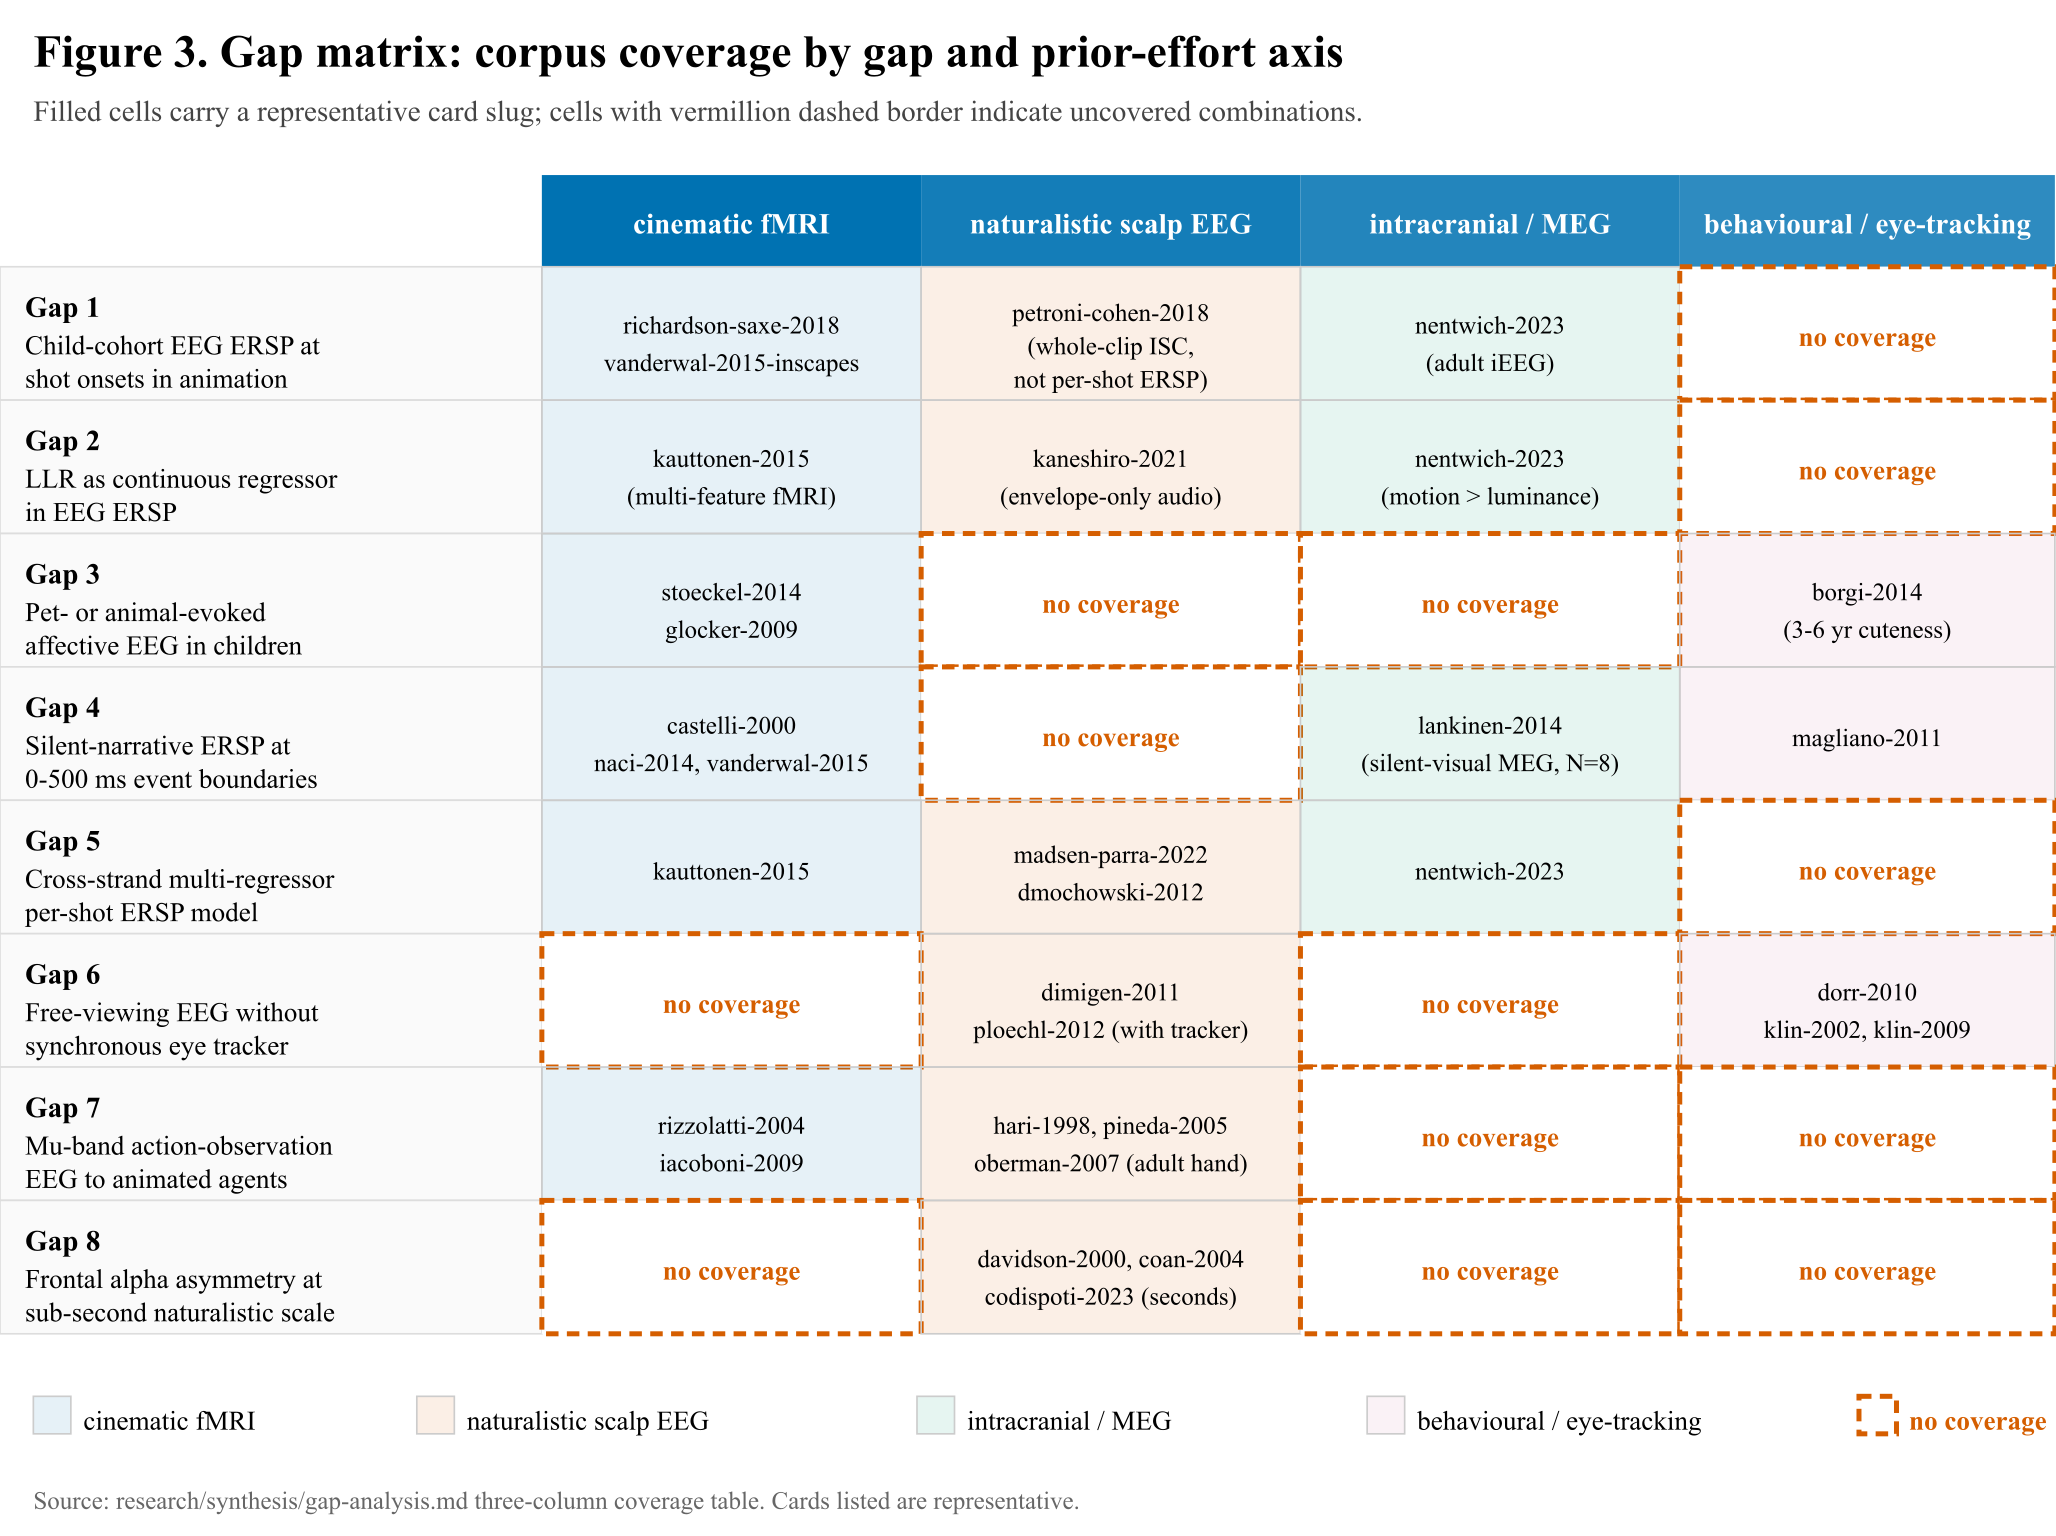
\includegraphics[width=\textwidth]{figures/fig3.png}
  \caption{\textbf{Gap matrix.} Eight named gaps from the four-strand corpus (rows) versus four prior-effort axes (cinematic fMRI, naturalistic scalp EEG, intracranial and MEG, behavioural and eye-tracking; columns). Filled cells list a representative card slug; cells marked ``no coverage'' with a vermillion dashed border indicate uncovered combinations. Thirteen cells across the eight rows carry no coverage, defining the design space for per-shot developmental EEG ERSP.}
  \label{fig:gap-matrix}
\end{figure}

\begin{figure}[h!]
  \centering
  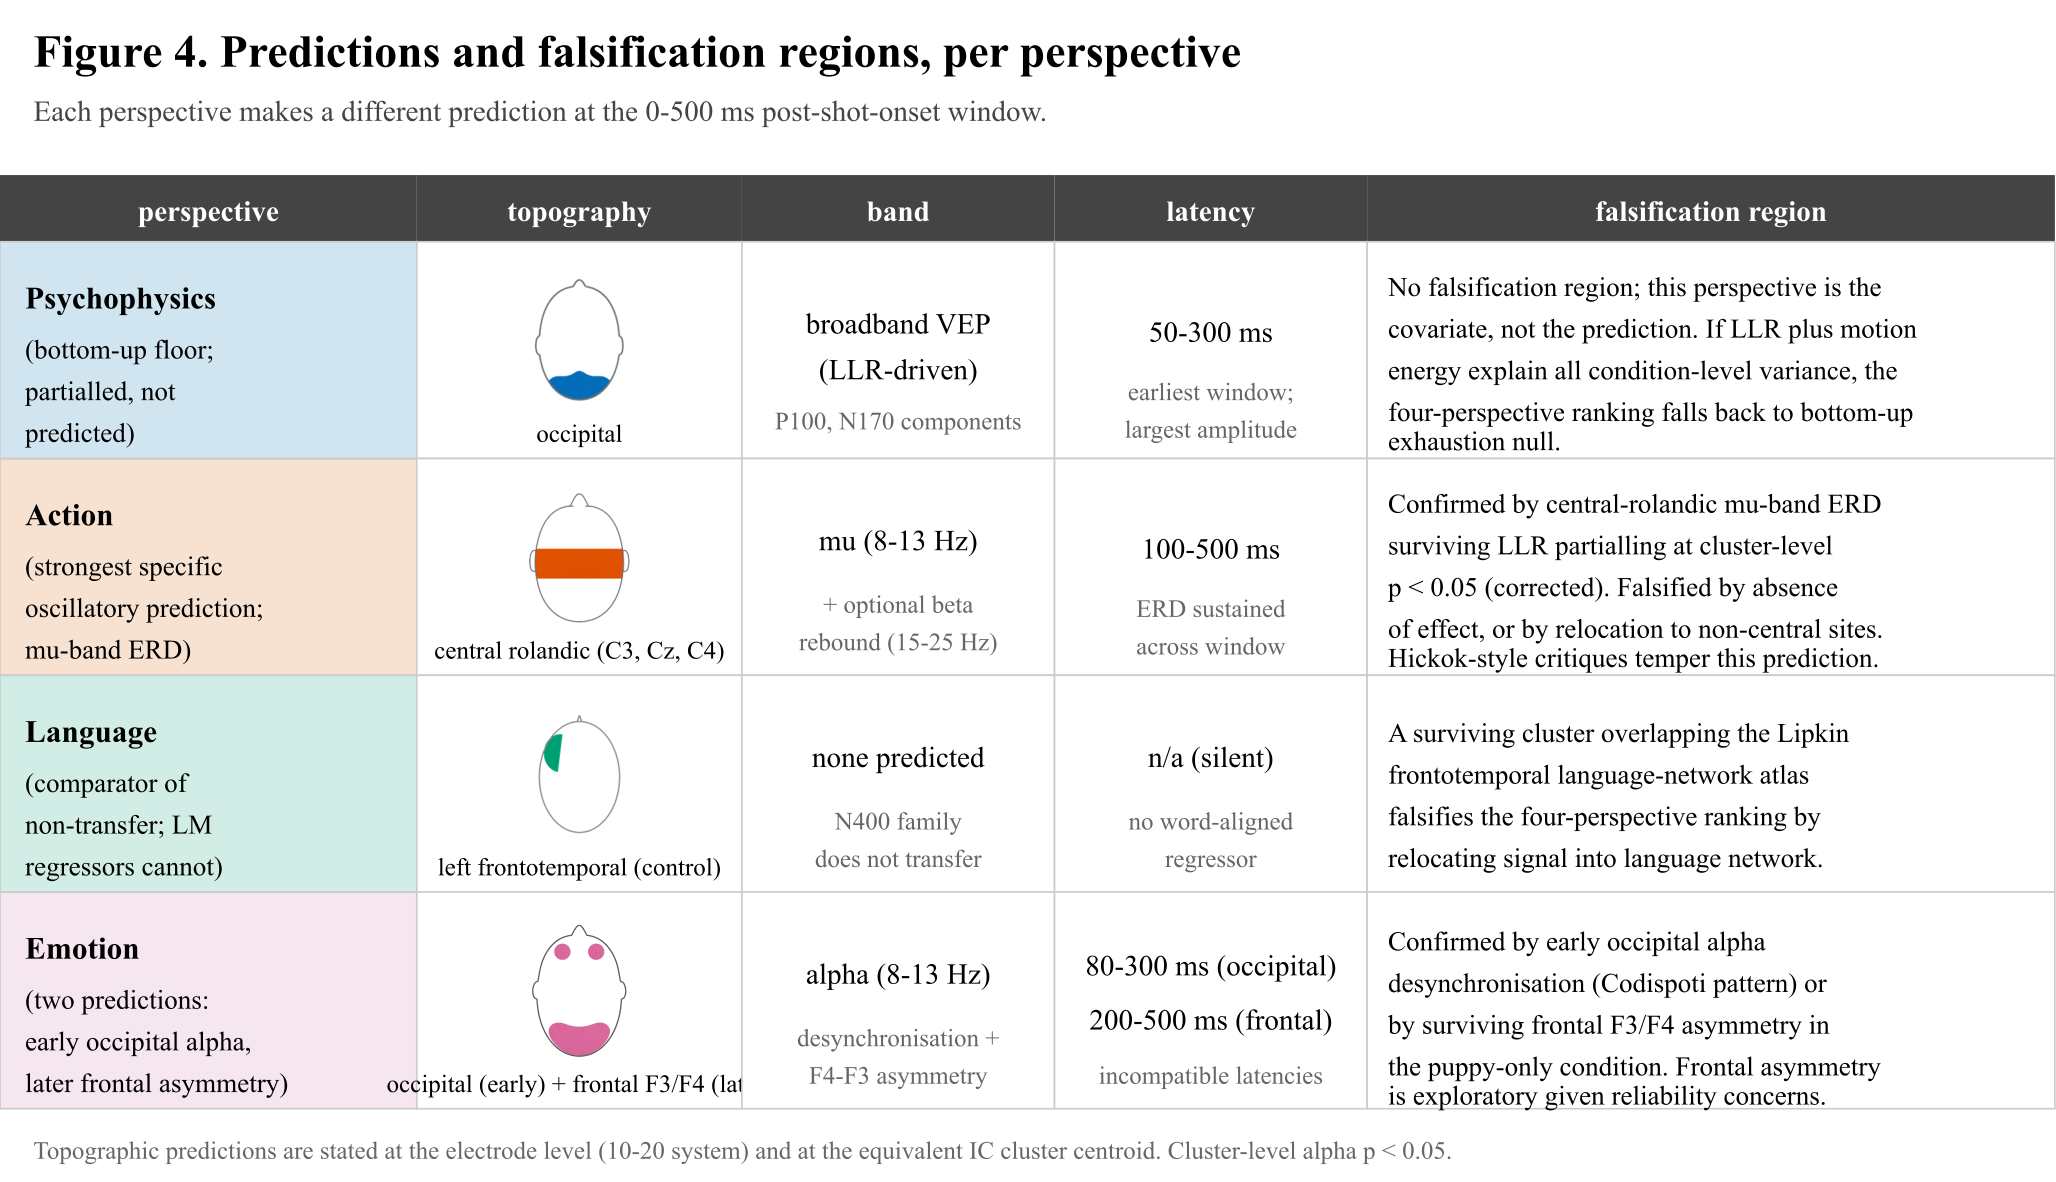
\includegraphics[width=\textwidth]{figures/fig4.png}
  \caption{\textbf{Predictions and falsification regions, per perspective.} Each perspective (row) is named with its predicted topography (with a head schematic showing the topographic focus), band, latency, and pre-registered falsification region. Psychophysics is the covariate, not the prediction. Action predicts central-rolandic mu-band (8 to 13 Hz) ERD over electrodes C3, Cz, and C4, with possible beta rebound (15 to 25 Hz). Language predicts no signal locally; a surviving cluster in left-frontotemporal IC space (Lipkin atlas negative-control mask) falsifies the four-perspective ranking. Emotion predicts early occipital alpha desynchronisation (80 to 300 ms) and later frontal F3/F4 asymmetry (200 to 500 ms), at incompatible latencies and topographies. The cluster-level alpha for falsification is $p < 0.05$ corrected by mass-univariate permutation.}
  \label{fig:predictions}
\end{figure}

\bibliography{refs}

\end{document}
